% !TeX root = 02gy_cpp
\documentclass[../cpp_book/cpp_book.tex]{subfiles}
\begin{document}
	\onlyinsubfile{
		\begin{center}
			{\LARGE\textbf{C++}}
			
			{\Large Gyakorlat jegyzet}
			
			2. óra
		\end{center}
		A jegyzetet \textsc{Umann} Kristóf készítette \textsc{Horváth} Gábor gyakorlata alapján. (\today)
	}
	\section{Láthatóság, élettartam}
	Egy objektum \textbf{láthatóságának} nevezzük a kódnak azon szakaszait, melyeknél lehet rá hivatkozni.
	\smallskip
	
	Egy objektum \textbf{élettartamának} nevezzük a kód azon szakaszát, melynél bent szerepel a memóriában. Amikor egy objektum élettartama elkezdődik, azt mondjuk, az objektum létrejön, míg az élettartam végén az objektum megsemmisül.
	\medskip
	\begin{note}
		Ez alapján megállapíthatjuk, hogy egy globális változó láthatósága és élettartama a program futásának elejétől végéig tart.
	\end{note}
	
	Figyeljük meg, mikor tudunk \texttt{x} változóra hivatkozni (azaz hol lesz \texttt{x} látható)!
	\begin{lstlisting}
int x;

int main()
{
	int x = 1;
	{
		int x = 2;
		std::cout << x << std::endl; // 2
	}
}
	\end{lstlisting}
	Megfigyelhető, hogy a \texttt{main} függvény elején létrehozott \texttt{x} az utána következő blokkban teljesen elérhetetlen -- nincs olyan szabványos nyelvi eszköz, amivel tudnánk rá hivatkozni. Ezt a folyamatot \textbf{leárnyékolás}nak (\textit{shadowing}) nevezzük. Azonban a külső, globális \texttt{x}-re bármikor tudunk hivatkozni az alábbi módon:
	\begin{lstlisting}
int x;

int main()
{
	int x = 1;
	{
		int x = 2;
		std::cout << ::x << std::endl; // 0
	}
}
	\end{lstlisting}
	\subsection{Jobb- és balérték}
	A láthatóság és élettartam fogalmával szoros összeköttetésben áll a \textbf{jobb- és balérték} fogalma. Egy objektumot \textbf{balértéknek} (\textit{left value}, röviden \textit{lvalue}) nevezzük, ha címképezhető, és \textbf{jobbértéknek} (\textit{right value}, röviden \textbf{rvalue}) ha nem. Példaképp:
	\begin{lstlisting}
int main()
{
	int *p, r; //balértékek
	&p; //ok, p pointer memóriacímére mutat
	&r; //ok, r memóriacímére mutat
	&5; //nem ok, 5 jobbérték
	&"Hello World!"; //nem ok, "Hello World!" jobbérték
	&&r; //nem ok, címképzés eredménye jobbérték
	5 = r; //nem ok, jobbértéknek nem lehet értéket adni
}
	\end{lstlisting}
	A jobbértékek többnyire ideiglenes objektumok, pl. egy érték szerint visszatérő függvény visszatérési értéke,  literálok mint pl. \texttt{5}, \texttt{"Hello World!"}. Lévén ezek az objektumok csak ideiglenesen szerepelnek a memóriában (sőt, gyakran egyáltalán nem, ha a fordító kioptimalizálja, ahogy azt korábban láthattuk), ezért hiba lenne a memóriacímükre hivatkozni, így a fordító ezt nem is engedi.
	\section{A stack működése}
	A stack a C++ alapértelmezett tárolási osztálya lokális változók esetén: minden változó alapértelmezetten itt jön létre és semmisül meg. Az itt létrejött változók automatikusan megsemmisülnek. Az élettartamuk a definíciójuktól az adott blokk végéig tart.
	
	\begin{lstlisting}
#include <iostream>

int f()
{
	int x = 0; //x létrejön
	++x;
	return x;
} //x megsemmisül

int main()
{
	for (int i = 0; i<5; i++)
		std::cout << f() << ' '; // 1 1 1 1 1
}
	\end{lstlisting}
	\medskip
	
	A fenti kód futása során a stack-et így képzelhetjük el:
	
	\begin{figure}[!h]
		\centering
		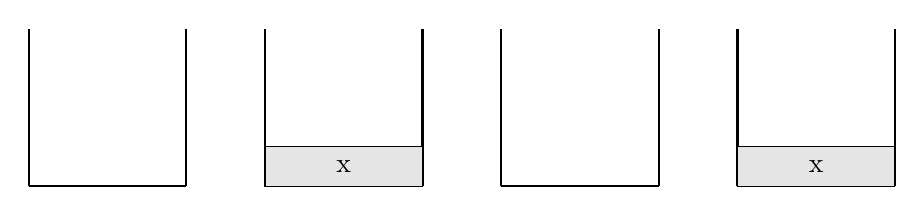
\begin{tikzpicture}
	\tikzstyle{Node} = [rectangle, minimum width=2cm, minimum height=5mm, text centered, draw=black, fill= gray!20]
	\tikzstyle{arrow} = [thick,->,>=stealth]
	
	
	\draw [thick, black] (-3, 0) -- (-1, 0);
	\draw [thick, black] (-3, 0) -- (-3, 2);
	\draw [thick, black] (-1, 0) -- (-1, 2);
	
	\draw [thick, black] (0, 0) -- (2, 0);
	\draw [thick, black] (0, 0) -- (0, 2);
	\draw [thick, black] (2, 0) -- (2, 2);
	\node (x) [Node] at (1,0.25) {x};
	
	\draw [thick, black] (3, 0) -- (5, 0);
	\draw [thick, black] (3, 0) -- (3, 2);
	\draw [thick, black] (5, 0) -- (5, 2);
	
	\draw [thick, black] (6, 0) -- (8, 0);
	\draw [thick, black] (6, 0) -- (6, 2);
	\draw [thick, black] (8, 0) -- (8, 2);
	\node (x) [Node] at (7,0.25) {x};
\end{tikzpicture}
		
		\smallskip
		\caption{}\label{fig_stack_example}
	\end{figure}
	Az ábrán egy stack-et látunk. Amikor a vezérlés az \texttt{f} függvényhez ér, és ott létrehozza az \texttt{x} változót, azt behelyezi a stack-be. A \texttt{return} kulcsszó hatására készít \texttt{x}-ről egy temporális példányt, ami a függvény visszatérési értéke lesz. Amikor a vezérlés visszatér a \texttt{main} függvényhez, {x}-re nem tudunk tovább hivatkozni, így azt megsemmisíti, és ez ismétlődik, ameddig a ciklus véget nem ér.
	\smallskip
	
	A stack egy FILO (\textit{first in last out}) adatszerkezet -- azaz azt az elemet ,,dobja'' ki a vezérlés a stack-ből, melyet utoljára rakott be.
	\section{Mutatók}
	A mutatók olyan nyelvi elemek, melyek egy adott típusú memóriaterületre mutatnak. Segítségükkel anélkül is tudunk hivatkozni egy adott objektumra (és nem csak a másolatára), hogy közvetlenül az objektummal dolgoznánk.
	\begin{lstlisting}
int main()
{
	int c = 5, d = 8;
	int *p = &c;
}
	\end{lstlisting}
	A fenti példában \texttt{p} egy mutató (\textit{pointer}), mely egy \texttt{int} típusra mutat. Ahhoz, hogy értéket tudjunk adni egy mutatónak, egy memóriacímet kell neki értékül adni, erre való a \textbf{címképző operátor} (\&). Ha a mutató által \textit{mutatott értéket} szeretnénk módosítani, akkor dereferálnunk kell a \textbf{dereferáló operátor}ral (*).
	
	A mutatók működését az alábbi példa demonstrálja:
	\begin{lstlisting}
int c = 5, d = 8;
int *p = &c; //referáljuk c-t
*p = 4; //dereferáljuk p-t
p = &d;
*p = 7;
	\end{lstlisting}
	\begin{figure}[!h]
		\centering
		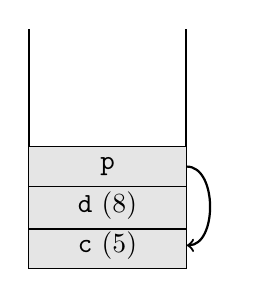
\begin{tikzpicture}
	\tikzstyle{Node} = [rectangle, minimum width=2cm, minimum height=5mm, text centered, draw=black, fill= gray!20]
	\tikzstyle{arrow} = [thick,->,>=stealth]
	
	\draw [thick, black] (0, 0) -- (2, 0);
	\draw [thick, black] (0, 0) -- (0, 3);
	\draw [thick, black] (2, 0) -- (2, 3);
	\node (c) [Node] at (1,0.25) {\texttt{c} (5)};
	\node (d) [Node] at (1,0.75) {\texttt{d} (8)};
	\node (p) [Node] at (1,1.25) {\texttt{p}};
	
	\path[every node/.style={font=\sffamily\small}]
	(p) edge[bend left = 90, thick, ->] node [right] {} (c);
\end{tikzpicture}\quad 
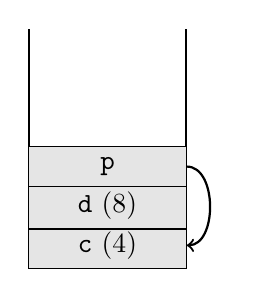
\begin{tikzpicture}
	\tikzstyle{Node} = [rectangle, minimum width=2cm, minimum height=5mm, text centered, draw=black, fill= gray!20]
	\tikzstyle{arrow} = [thick,->,>=stealth]
	
	\draw [thick, black] (0, 0) -- (2, 0);
	\draw [thick, black] (0, 0) -- (0, 3);
	\draw [thick, black] (2, 0) -- (2, 3);
	\node (c) [Node] at (1,0.25) {\texttt{c} (4)};
	\node (d) [Node] at (1,0.75) {\texttt{d} (8)};
	\node (p) [Node] at (1,1.25) {\texttt{p}};
	
	\path[every node/.style={font=\sffamily\small}]
	(p) edge[bend left = 90, thick, ->] node [right] {} (c);
\end{tikzpicture}\quad 
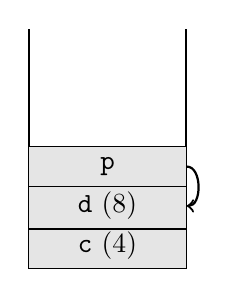
\begin{tikzpicture}
	\tikzstyle{Node} = [rectangle, minimum width=2cm, minimum height=5mm, text centered, draw=black, fill= gray!20]
	\tikzstyle{arrow} = [thick,->,>=stealth]
	
	\draw [thick, black] (0, 0) -- (2, 0);
	\draw [thick, black] (0, 0) -- (0, 3);
	\draw [thick, black] (2, 0) -- (2, 3);
	\node (c) [Node] at (1,0.25) {\texttt{c} (4)};
	\node (d) [Node] at (1,0.75) {\texttt{d} (8)};
	\node (p) [Node] at (1,1.25) {\texttt{p}};
	
	\path[every node/.style={font=\sffamily\small}]
	(p) edge[bend left = 90, thick, ->] node [right] {} (d);
\end{tikzpicture}\quad 
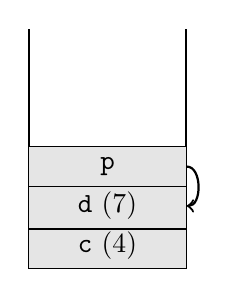
\begin{tikzpicture}
	\tikzstyle{Node} = [rectangle, minimum width=2cm, minimum height=5mm, text centered, draw=black, fill= gray!20]
	\tikzstyle{arrow} = [thick,->,>=stealth]
	
	\draw [thick, black] (0, 0) -- (2, 0);
	\draw [thick, black] (0, 0) -- (0, 3);
	\draw [thick, black] (2, 0) -- (2, 3);
	\node (c) [Node] at (1,0.25) {\texttt{c} (4)};
	\node (d) [Node] at (1,0.75) {\texttt{d} (7)};
	\node (p) [Node] at (1,1.25) {\texttt{p}};
	
	\path[every node/.style={font=\sffamily\small}]
	(p) edge[bend left = 90, thick, ->] node [right] {} (d);
\end{tikzpicture}
		
		\smallskip
		\caption{Az objektum neve mellett zárójelben található az értéke.}\label{fig_stack_pointer_intro}
	\end{figure}
	Rendre: pointer inicializálása, pointer által mutatott érték módosítása, pointer átállítása másik memóriacímre, és a mutatott érték módosítása.
	
	Egy mutató mutathat változóra, másik mutatóra vagy sehova. Azokat a mutatókat, melyek sehová sem mutatnak, null pointernek nevezzük, és így hozhatjuk létre őket:
	
	{\centering \texttt{p = 0;\quad \quad p = NULL;\quad \quad p = nullptr;} \par}
	\begin{note}
		Ez a három értékadás (közel) ekvivalens, azonban a \texttt{nullptr} kulcsszó csak C++11ben és azutáni szabványokban érhető el.
	\end{note}
	\subsection{Konstans korrektség}
	A konstans korrektség egy szabály a C++ nyelvben: ha egy értéket konstansnak jelölünk, azt nem módosíthatjuk a program futása során.
	\begin{lstlisting}
const int ci = 6;
int *p = &ci;
	\end{lstlisting}
	A fenti kód nem fordul le, mert \texttt{ci} konstans, de \texttt{p} nem egy nem konstans\textbf{ra} mutató mutató, ugyanis ez sérteni a konstans korrektséget. A probléma forrása az, ha fenti értékadás lefordulna, akkor \texttt{ci} értékét tudnánk módosítani \texttt{p}-n keresztül.
	\begin{lstlisting}
const int ci = 6;
const int *p = &ci;
	\end{lstlisting}
	A fenti módosítással a kód már lefordul, hiszen a \texttt{p} itt már egy konstansra mutató mutató, azaz mutathat konstans változókra. Egy konstansra mutató mutató \textbf{nem tudja megváltoztatni} a mutatott értéket, viszont át lehet állítani egy másik memóriacímre.
	\begin{lstlisting}
const int ci = 6;
const int *p = &ci;

int c = 5;
p = &c;
	\end{lstlisting}
	A fenti kód is szabályos, konstansra mutató mutatóval nem konstans is értékre mutathatunk. Érdemes átgondolni ennek a következményeit, hisz \texttt{c} nem konstans, ezért az értékét továbbra is módosíthatjuk (csak nem \texttt{p}-n keresztül)! Egy konstansra mutató mutató nem azt jelenti, hogy a mutatott érték sosem változhat meg. Csupán annyit jelent, hogy a mutatott értéket ezen a mutatón keresztül nem lehet megváltoztatni.
	\begin{lstlisting}
const int *p = &ci;
int c = 5;
p = &c;
c = 5;
	\end{lstlisting}
	A \texttt{const} kulcsszó több helyre is kerülhet.
	\begin{lstlisting}
const int *p;
int const *p;
	\end{lstlisting}
	A fenti két sor ugyanazt jelenti, a mutatott értéket nem lehet megváltoztatni a mutatón keresztül.
	\begin{lstlisting}
int * const p;
	\end{lstlisting} 
	Amennyiben a * után van a \texttt{const}, akkor egy \textbf{konstans mutatót kapunk}, mely megváltoztathatja a mutatott értéket, de nem mutathat másra (konstans mutató\quad$\not=$\quad konstanra mutató mutató). Nyilván, egy pointer lehet egy konstansra mutató konstans mutató is, amin keresztül nem lehet megváltoztatni a mutatott értéket és a mutatót sem lehet máshova átállítani.
	\begin{lstlisting}
const int * const p;
	\end{lstlisting}
	\subsection{Mutatóra mutató mutatók} 
	Mutatóra mutató mutatók is léteznek. Néhány példa:
	\begin{lstlisting}
int *p;
int **q = &p;
int ***r = &q;
	\end{lstlisting}
	Példaképp \texttt{q}-n keresztül meg tudjuk változni, \texttt{p} hova mutasson.
	\begin{lstlisting}
int c, d;
int *p = &c;
int **q = &p;
*q = &d;
	\end{lstlisting}
	A megfelelő szinten a mutatók konstansá tételével még bonyolultabb példákat kaphatunk:
	\begin{lstlisting}
int c, d;
int *p = &c;
int * const *q = &p;
*q = &d; // forditasi hiba
	\end{lstlisting}
	Mivel \texttt{q} egy \texttt{int}-re mutató konstans mutatóra mutató mutató, így csak egy olyan mutatóval tudunk rámutatni, ami egy \texttt{int}-re mutató konstans mutatóra mutató mutatóra mutató mutató.
	\begin{lstlisting}
int c, d;
int *p = &c;
int * const *q = &p;
int *const ** const r = &q;
	\end{lstlisting}
	\begin{note}
		Megnyugtatás végett, ritkán van szükség mutatóra mutató mutatónál bonyolultabb szerkezetre.
	\end{note}\section{Tömbök}
	A tömb a C++ egy beépített adatszerkezete, mellyel tömb azonos típusú elemet tárolhatunk és kezelhetünk egységesen. Előzménytárgyakból már megismertük valamennyi funkcionalitását, ám számos veszélyét még nem.
	\begin{lstlisting}
int main()
{
	int i = 5;
	int t[] = {5,4,3,2,1};
}
	\end{lstlisting}
	\texttt{t} egy 5 elemű \textbf{tömb}. Nézzük meg, mekkora a mérete (figyelem, ez \textbf{implementációfüggő!})!
	\begin{lstlisting}
std::cout << sizeof(i) << std::endl;
std::cout << sizeof(t) << std::endl;
	\end{lstlisting}
	A \texttt{sizeof} operátor megadja a paraméterként megadott típus, vagy objektum esetében annak típusának méretét (bővebben később). Ez minden implementációra specifikus. Azt látjuk, hogy mindig ötszöröse lesz a \texttt{t} az \texttt{i}-nek. Azaz a tömbök tiszta adatok.  Stacken ábrázolva így képzeljük el:
	
	\begin{figure}[!h]
		\centering
		\begin{tikzpicture}
	\drawStackFrame{0}{0}{3.5}
	\node (c2) [StackObject] at (1,0.25) {\texttt{i} (5)};
	\node (d2) [StackObject] at (1,0.75) {\texttt{t[0]} (5)};
	\node (d2) [StackObject] at (1,1.25) {\texttt{t[1]} (4)};
	\node (d2) [StackObject] at (1,1.75) {\texttt{t[2]} (3)};
	\node (d2) [StackObject] at (1,2.25) {\texttt{t[3]} (2)};
	\node (d2) [StackObject] at (1,2.75) {\texttt{t[4]} (1)};
\end{tikzpicture}
		
		\caption{A \texttt{main} függvény változói.}\label{fig_stack_array}
	\end{figure}
	\subsection{Biztonsági rések nem definiált viselkedés kihasználásával}
	Irassuk ki a a tömb elemeit! A példa kedvéért rontsuk el a kódot.
		\begin{lstlisting}
for (int i = 0; i < 6; i++) // Hupsz. A csak 5 elem van.
{
	std::cout << t[i] << std::endl;
}
	\end{lstlisting} 
	Itt látható, hogy túl fogunk indexelni. Ez {nem definiált viselkedés}hez vezet. Várhatóan memóriaszemetet fog kiolvasni az utolsó elem helyett, de sose tudhatjuk pontosan mi fog történni. Fordítási időben ezt a hibát a fordító nem veszi észre. A gyakorlaton a programot futtatva nem következett be futási idejű hiba.
	
	Most növeljük meg az elemeket, és indexeljünk túl egészen 100ig!
	\begin{lstlisting}
for (int i = 0; i < 100; i++)
{
	++t[i];
}
std::cout << "sajt" << std::endl;
	\end{lstlisting} 
	Ez a program továbbra is nem definiált viselkedést tartalmaz. Mivel több memóriához nyúlunk hozzá indokolatlanul, ezért nagyobb rá az esély, hogy futási idejű hibába ütközzünk. Az órán a {sajt} szöveg ki lett írva, mégis kaptunk egy szegmentálási hibát (\textit{segmentation fault}).
	
	\begin{lstlisting}
for (int i = 0; i < 100000; i++)
{
	++t[i];
}
std::cout << "sajt" << std::endl;
	\end{lstlisting} 
	A túlindexelést tovább fokozva a program még mielőtt sajt-ot ki tudta volna írni, szegmentálási hibával leállt. Ez jól demonstrálja, hogy ugyanolyan jellegű  a hibát követtük el, de mégis más volt a végeredmény. Ez az egyik ok, amiért veszélyesek a nem definiált viselkedések. Mivel számos különböző hibát okozhatnak, ezért a diagnosztizálásuk sem mindig egyszerű. Az alábbi kód szemléltet egy példát, hogyan lehet biztonsági rés a nem definiált viselkedésből.
	\begin{lstlisting}
#include <iostream>
#include <string>

int main()
{
	int t[] = {5,4,3,2,1};
	int isAdmin = 0;
	std:string name;
	std::cin >> name;
	for (int i = 0; i < name.size(); ++i)
	{
		t[i] = 1;
	}
	if (name == "pityu")
		isAdmin = 1;
	std::cout << "Admin?: " << (isAdmin != 0 ) << std::endl;
}
	\end{lstlisting}
	Ha a programnak \texttt{pityu}-t adunk meg amikor be akarja olvasni \texttt{name}-et, akkor minden rendben. De mivel a forráskódot ismerjük, azért ha hosszú nevet adnánk (nagyobb mint 5), akkor a túlindexelés miatt ki tudjuk használni a nem definiált viselkedéseket. Az is előfordulhat, hogy az \texttt{isAdmin} memóriacímére írunk, és elérjük, hogy a szoftver adminként authentikáljon valakit, aki nem az.
	\medskip
	
	Hogyan lehet ezeket a hibákat elkerülni? Túl azon, hogy figyelni kell, vannak programok amik segítenek. Ehhez használhatunk \texttt{sanitizer}-eket. Ezek módosítanak a fordító által generált kódon. Létrehoz ellenőrzéseket, amik azelőtt észrevesznek bizonyos nem definiált viselkedéseket, mielőtt azok megtörténnének. Pl. itt a túlindexelés, egy futási idejű hibához és egy jól olvasható hibaüzenethez vezetne. Használatukhoz elég egy extra paranccsal fordítanunk:
	
	{\centering\texttt{g++ main.cpp -fsanitize=address}\par }
	
	A sanitizerek csa abban az esetben találnak meg egy hibát, ha a probléma előfordul (azaz futási időben, nem fordítási időben ellenőriz). Amennyiben előfordul, akkor elég pontos leírást tudunk kapni arról, hogy merre van a probléma. Fordítási időben a figyelmeztetések használata segíthet bizonyos hibák elkerülésében.
	
	{\centering \texttt{g++ main.cpp -Wall -Wextra} \par}
	
	A fenti két kapcsoló szintén extra ellenőrzéseket vezet be, de nem változtatják meg a generált kódot.
	\subsection{Hivatkozás tömb elemeire}
	Egy tömb adott elemére több módon is hivatkozhatunk:
	
	{\centering \texttt{*(p + 3) == *(3 + p) == p[3] == 3[p]} \par}
	\
	\begin{lstlisting}
#include <iostream>

int main()
{
	int t[][3] = {{1,2,3},{4,5,6}};
	return 0;
}
	\end{lstlisting}
	Tekintsük a fenti két dimenziós tömböt. Az első \texttt{[]} jelek közt nincs méret, mert a fordító az inicializáció alapján meg tudja állapítani. A második dimenzió méretének megadása viszont kötelező.
	
	\medskip
	Fentebb a tömböknél megadott ekvivalenciát a mátrixra alkalmazva számos indexelési módot le tudunk vezetni:
	\medskip
	
	\begin{center}
		\texttt{t[1][] == *(*(t+1)+0) == *(1[t]+0) == 0[1[t]] == 0[*(t+1)] == *(t+1)[0] == 1[t][0] } 
		\end{center}
	\begin{note}
		Előzmény tárgyakból elképzelhető, hogy azt tanultuk, hogy egy tömb méretének egy változót is megadhatunk. Ezt a \texttt{gcc} fordító elfogadja és jó kódot is generál belőle. De ez egy nem szabványos kiterjesztés, ezért nem garantált, hogy ezt minden fordító megteszi. Ez jól demonstrálja, hogy a fordítók nem mindenben követik szorosan a szabványt.
	\end{note}
	\section{Paraméter átvétel, visszatérési érték}
	\subsection{Érték szerinti paraméter átvétel}
	C++ban alapértelmezett módon a paraméterátadás érték szerint történik. Figyeljük meg ennek a következményét a \texttt{swap} függvény megvalósításával!
	%http://tex.stackexchange.com/questions/228724/how-do-i-make-tikz-make-a-curved-arrow-from-one-node-to-another-when-my-nodes-ar
	\begin{lstlisting}
#include <iostream>
void swapWrong(int a, int b)
{
	int tmp = a;
	a = b;
	b = tmp;
}

int main()
{
	int c = 5, d = 8;
	swapWrong(c, d);
	std::cout << c << ' ' << d << std::endl; //5 8
}
	\end{lstlisting}		
	Megfigyelhető, hogy nem sikerült \texttt{c} és \texttt{d} értékét megcserélni. Ez azonban egy teljesen jól definiált viselkedés. Ennek az az oka, hogy itt \textbf{érték} szerint vettük át (\textit{pass by value}) \texttt{a} és \texttt{b} paramétert. A következő ábrán megfigyelhetjük mi is történik pontosan. Képzeljük el, hogy a stackbe a program elrakja a \texttt{c} és \texttt{d} változókat. Eztán meghívja a \texttt{swapWrong} függvényt, melyben létrehozott \texttt{a} és \texttt{b} paraméterek szintén a stackre kerülnek. Bár a függvényre lokális \texttt{a} és \texttt{b} paraméterek értékét megcseréli, de a függvényhívás után ezeket ki is törli a stackből. Az eredeti \texttt{c} és \texttt{d} változók éréke nem változott a függvényhívás során. (ld.: \ref{fig_stack_swap_wrong}. ábra)
	\begin{figure}[!h]
		\centering
		\begin{tikzpicture}
	\drawStackFrame{0}{0}{3};
	\node (c2) [StackObject] at (1,0.25) {\texttt{c} (5)};
	\node (d2) [StackObject] at (1,0.75) {\texttt{d} (8)};
	
	\drawStackFrame{3}{0}{3};
	\node (c3) [StackObject] at (4,0.25) {\texttt{c} (5)};
	\node (d3) [StackObject] at (4,0.75) {\texttt{d} (8)};
	\node (a3) [StackObject] at (4,1.25) {\texttt{a} (5)};
	\node (b3) [StackObject] at (4,1.75) {\texttt{b} (8)};
	\node (b3) [StackObject] at (4,2.25) {\texttt{tmp} (5)};
	
	\drawStackFrame{6}{0}{3};
	\node (c3) [StackObject] at (7,0.25) {\texttt{c} (5)};
	\node (d3) [StackObject] at (7,0.75) {\texttt{d} (8)};
	\node (a3) [StackObject] at (7,1.25) {\texttt{a} (8)};
	\node (b3) [StackObject] at (7,1.75) {\texttt{b} (5)};
	\node (b3) [StackObject] at (7,2.25) {\texttt{tmp} (5)};
	
	\drawStackFrame{9}{0}{3};
	\node (a4) [StackObject] at (10,0.25) {\texttt{c} (5)};
	\node (b4) [StackObject] at (10,0.75) {\texttt{d} (8)};
\end{tikzpicture}
		
		\caption{A \texttt{swapWrong} függvény szemléltetése a stack-en.}\label{fig_stack_swap_wrong}
	\end{figure}
	\subsection{Mutatók érték szerinti átadása}
  	Nézzük meg, hogy hogyan tudunk megcserélni két értéket ezúttal helyesen, mutatók segítségével.
	
	\begin{lstlisting}
void swapP(int *a, int *b)
{
	int tmp = *a;
	*a = *b;
	*b = tmp;
}
	\end{lstlisting}
	
	Amennyiben ezt a függvényt hívjuk meg, valóban megcserélődik a két változó értéke. De ehhez fontos, hogy ne \texttt{swapP(c, d)}-t írjunk, az ugyanis az fordítási hibához vezetne, hiszen a \texttt{c} és \texttt{d} típusa \texttt{int}, és nem \texttt{int*}. Ahhoz, hogy értéket adjunk egy pointernek, a \texttt{c}-hez és \texttt{d}-hez tartozó memóriacímeket kell átadni!
	\begin{lstlisting}
//...
int main()
{
	int c = 5, d = 8;
	swapP(&c, &d);
	std::cout << c << ' ' << d << std::endl; // 8 5
}
	\end{lstlisting}
	\begin{note}
    A mutatókat továbbra is érték szerint adjuk át. Az \texttt{a} és \texttt{b} paraméterekben lévő memóriacím tehát a másolata annak, amit a hívás helyén megadtunk.
	\end{note}
	\begin{figure}[!h]
		\centering
		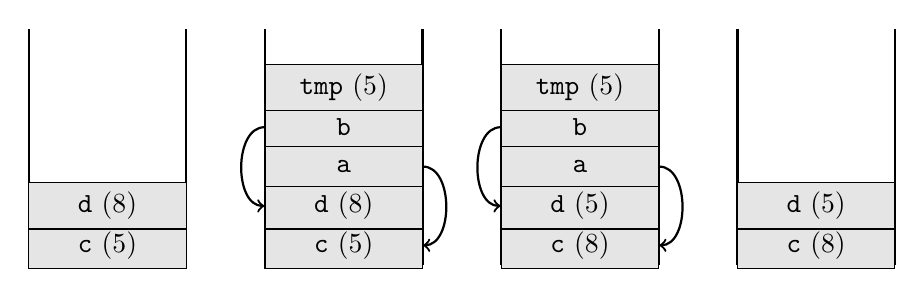
\begin{tikzpicture}
	\tikzstyle{Node} = [rectangle, minimum width=2cm, minimum height=5mm, text centered, draw=black, fill= gray!20]
	\tikzstyle{arrow} = [thick,->,>=stealth]
	
	\draw [thick, black] (-3, 0) -- (-1, 0);
	\draw [thick, black] (-3, 0) -- (-3, 3);
	\draw [thick, black] (-1, 0) -- (-1, 3);
	\node (c1) [Node] at (-2,0.25) {\texttt{c} (5)};
	\node (d1) [Node] at (-2,0.75) {\texttt{d} (8)};
	
	\draw [thick, black] (0, 0) -- (2, 0);
	\draw [thick, black] (0, 0) -- (0, 3);
	\draw [thick, black] (2, 0) -- (2, 3);
	\node (c2) [Node] at (1,0.25) {\texttt{c} (5)};
	\node (d2) [Node] at (1,0.75) {\texttt{d} (8)};
	\node (a2) [Node] at (1,1.25) {\texttt{a}};
	\node (b2) [Node] at (1,1.75) {\texttt{b}};
	\node (tmp2) [Node] at (1,2.25) {\texttt{tmp} (5)};
	
	\path[every node/.style={font=\sffamily\small}]
		(a2) edge[bend left = 90, thick, ->] node [right] {} (c2);
	\path[every node/.style={font=\sffamily\small}]
		(b2) edge[bend right = 90, thick, ->] node [left] {} (d2);
	
	\draw [thick, black] (3, 0) -- (5, 0);
	\draw [thick, black] (3, 0) -- (3, 3);
	\draw [thick, black] (5, 0) -- (5, 3);
	\node (c3) [Node] at (4,0.25) {\texttt{c} (8)};
	\node (d3) [Node] at (4,0.75) {\texttt{d} (5)};
	\node (a3) [Node] at (4,1.25) {\texttt{a}};
	\node (b3) [Node] at (4,1.75) {\texttt{b}};
	\node (tmp3) [Node] at (4,2.25) {\texttt{tmp} (5)};
	
	
	\path[every node/.style={font=\sffamily\small}]
	(a3) edge[bend left = 90, thick, ->] node [right] {} (c3);
	\path[every node/.style={font=\sffamily\small}]
	(b3) edge[bend right = 90, thick, ->] node [left] {} (d3);
	
	\draw [thick, black] (6, 0) -- (8, 0);
	\draw [thick, black] (6, 0) -- (6, 3);
	\draw [thick, black] (8, 0) -- (8, 3);
	\node (a4) [Node] at (7,0.25) {\texttt{c} (8)};
	\node (b4) [Node] at (7,0.75) {\texttt{d} (5)};
\end{tikzpicture}
		
		\caption{A \texttt{swapP} függvény szemléltetése.}\label{fig_stack_swap_p}
	\end{figure}
	
	\begin{lstlisting}
void swapWrong2(int *a, int *b)
{
	int *tmp = a;
	a = b;
	b = tmp;
}
	\end{lstlisting}
	Ebben a példában nem a pointerek által mutatott értéket, hanem magukat a pointereket cseréljük meg. Itt az fog történni, hogy a függvény belsejében \texttt{a} és \texttt{b} pointer másra fog mutatni. A mutatott értékek viszont nem változnak.
	
	\begin{figure}[!h]
		\centering
		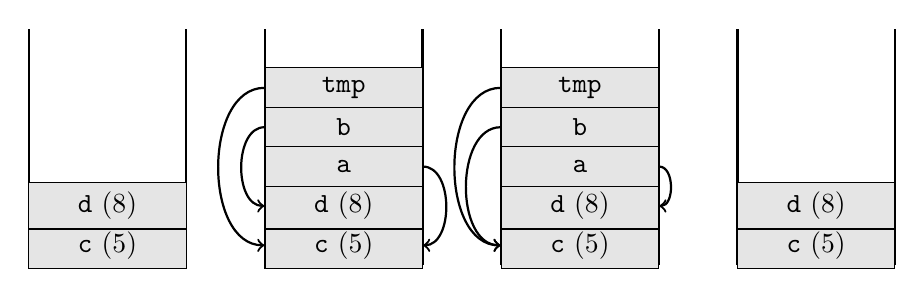
\begin{tikzpicture}
	\tikzstyle{Node} = [rectangle, minimum width=2cm, minimum height=5mm, text centered, draw=black, fill= gray!20]
	\tikzstyle{arrow} = [thick,->,>=stealth]
	
	\draw [thick, black] (-3, 0) -- (-1, 0);
	\draw [thick, black] (-3, 0) -- (-3, 3);
	\draw [thick, black] (-1, 0) -- (-1, 3);
	\node (c1) [Node] at (-2,0.25) {\texttt{c} (5)};
	\node (d1) [Node] at (-2,0.75) {\texttt{d} (8)};
	
	\draw [thick, black] (0, 0) -- (2, 0);
	\draw [thick, black] (0, 0) -- (0, 3);
	\draw [thick, black] (2, 0) -- (2, 3);
	\node (c2) [Node] at (1,0.25) {\texttt{c} (5)};
	\node (d2) [Node] at (1,0.75) {\texttt{d} (8)};
	\node (a2) [Node] at (1,1.25) {\texttt{a}};
	\node (b2) [Node] at (1,1.75) {\texttt{b}};
	\node (tmp2) [Node] at (1,2.25) {\texttt{tmp}};
	
	\path[every node/.style={font=\sffamily\small}]
	(a2) edge[bend left = 90, thick, ->] node [right] {} (c2);
	\path[every node/.style={font=\sffamily\small}]
	(b2) edge[bend right = 90, thick, ->] node [left] {} (d2);
	\path[every node/.style={font=\sffamily\small}]
	(tmp2) edge[bend right = 90, thick, ->] node [left] {} (c2);
	
	\draw [thick, black] (3, 0) -- (5, 0);
	\draw [thick, black] (3, 0) -- (3, 3);
	\draw [thick, black] (5, 0) -- (5, 3);
	\node (c3) [Node] at (4,0.25) {\texttt{c} (5)};
	\node (d3) [Node] at (4,0.75) {\texttt{d} (8)};
	\node (a3) [Node] at (4,1.25) {\texttt{a}};
	\node (b3) [Node] at (4,1.75) {\texttt{b}};
	\node (tmp3) [Node] at (4,2.25) {\texttt{tmp}};
	
	
	\path[every node/.style={font=\sffamily\small}]
	(a3) edge[bend left = 90, thick, ->] node [right] {} (d3);
	\path[every node/.style={font=\sffamily\small}]
	(b3) edge[bend right = 90, thick, ->] node [left] {} (c3);
	\path[every node/.style={font=\sffamily\small}]
	(tmp3) edge[bend right = 90, thick, ->] node [left] {} (c3);
	
	\draw [thick, black] (6, 0) -- (8, 0);
	\draw [thick, black] (6, 0) -- (6, 3);
	\draw [thick, black] (8, 0) -- (8, 3);
	\node (a4) [Node] at (7,0.25) {\texttt{c} (5)};
	\node (b4) [Node] at (7,0.75) {\texttt{d} (8)};
\end{tikzpicture}
		
		\caption{A \texttt{swapWrong2} függvén szemléltetése.}\label{fig_stack_swap_wrong_2}
	\end{figure}
	\subsection{Referencia szerinti paraméter átadás}
	Megállapíthatjuk, hogy az előző megoldásnál nem változtattuk meg, hogy mire mutassanak a pointerek, így azokat konstansként is definiálhatnánk. A konstans pointerek módosíthatják a mutatott értéket, de nem lehet őket átállítani egy másik memória címre. Úgy tudunk egy ilyen pointert létrehozni, hogy a csillag után írjuk a \texttt{const} kulcsszót.
	\begin{lstlisting}
void swap(int * const a, int * const b)
{
	//...
}
	\end{lstlisting}
	Egy kis szintaktikai cukorkával megúszhatjuk azt, hogy folyton kiírjuk a \texttt{* const}-ot (lévén nem akarjuk megváltoztatni, hogy ilyen esetben a pointer hova mutasson). Erre való a {referencia szerinti paraméter átváétel} (\textit{pass by reference}). A referencia hasonlóan működik, mintha egy konstans pointer lenne, csak nem lehet sehova se mutató referenciát létrehozni.
	\begin{lstlisting}
void swapRef(int &a, int &b)
{
	int tmp = a;
	a = b;
	b = tmp;
}
	\end{lstlisting} 
  Ez a függvény lényegében ekvivalens a \texttt{swapP} fügvénnyel. 
	\begin{note}
		Ez bár ezt referencia szerinti átvételnek nevezzük, de itt is történik másolás, a memóriacímet ítt is érték szerint vesszük át.
	\end{note}
		Megjegyzendő, hogy a fenti \texttt{swapRef} függvény meghívásakor nem kell jeleznünk, hogy memóriacímeket akarunk átadni, \texttt{swapRef(a,b)}-t kell írnunk.
	\begin{note}
		Egy referenciát mindig inicializálni kell. Csak úgy mint egy konstanst (különben fordítási hibát kapunk.)
	\end{note}
	\subsection{Visszatérési érték problémája}
	Nem primitív (pl. \texttt{int}) típusoknál gyakran megeshet, hogy egy adott típushoz tartozó pointer mérete kisebb, mint magának az objektumé, így megérheti mindentől függetlenül a paramétert referencia szerint átvenni. Ezen felbátorodva mondhatnánk azt is, hogy referenciával is térjünk vissza (a követekező példában tekintsünk el attól, hogy \texttt{int}-el dolgozunk, bátran képzeljük azt hogy az pl. egy nagyon nagy mátrix)!
	\begin{lstlisting}
int& addOne(int &i)
{
	i++;
	return i;
}

int main()
{
	int i = 0;
	int a = addOne(i);
	std::cout << a << std::endl;
}
	\end{lstlisting}
	A fenti kóddal semmi gond nincs is. De mi van, ha egy picit módosítunk rajta?
	\begin{lstlisting}
int& addOne(int &i)
{
	int ret = ++i;
	return ret;
}
	\end{lstlisting}
	A baj máris megvan, amit egy warning is jelezni fog nekünk: olyan objektumra hivatkozó referenciát adunk vissza, amely \texttt{addOne}-on belül lokális. Ez azt jelenti, hogy amint a vezérlés visszatér a \texttt{main} függvényhez, \texttt{ret} megsemmisül, és a \texttt{main} függvény pedig a \texttt{ret}-hez tartozó címen lévő értéket próbálná meg lemásolni. Mivel viszont a \texttt{ret} már ezen a ponton megsemmisült, semmi nem garantálja, hogy azon a memóriaterületen ne követekezett volna be módosítás.
	
	\medskip
	Az olyan memóriaterületre való hivatkozás, mely nincs a program számára lefoglalva, nem definiált viselkedést eredményez.
	\begin{note}
		Értelemszerűen pointerekkel ez ugyanúgy probléma.
	\end{note}
	\subsection{Függvények átadása paraméterként}
	C++ban lehetőségünk van arra is, hogy függvényeket adjunk át paraméterként. Azokat az objektumokat függvény mutatónak (\textit{function pointer}) hívjuk.
	\begin{lstlisting}
int add(int a, int b)
{
	return a + b;
}

int mul(int a, int b)
{
	return a * b;
}

int reduce(int *start, int size, int initial, int (*op)(int, int))
{
	int ret = initial;
	for (int i = 0; i < size; i++)
	{
		ret = (*op)(ret, start[i]);
	}
	return ret;
}

int main()
{
	int t[] = {1,2,3,4,5};
	std::cout << reduce(t,5,0,&add) << std::endl;
	std::cout << reduce(t,5,0,&mul) << std::endl;
}
	\end{lstlisting}
	
	Itt \texttt{reduce} egy olyan paramétert is vár, mely igazából egy függvény, amely \texttt{int}-et ad vissza, és két \texttt{int}-et vár paraméterül.
	\begin{note}
		A szavakba öntés segíthet a megértésben: \texttt{op} egy olyan függvényre mutató mutató, melynek két \texttt{int} paramétere van, és \texttt{int} a visszatérési értéke.
	\end{note}
	
	A kódban feltűnhet, hogy a tömb mellé paraméterben elkértük annak méretét is. Ennek az az oka, hogy a \texttt{t} tömb egy \texttt{int}-re mutató mutatóvá fog konvertálódni a paraméter átadás során, ami a tömb első elemére mutat. Ennek hatására elvesztjük azt az információt, hogy mekkora volt a tömb (a tömbök és paraméterátadás kapcsolátról később bévebben lesz szó). Így át kell adni ezt az információt is. 
	
	Mellékesen, egy függvény átadásakor csak függvénypointert tudunk átadni. Egy függvénypointeren a függvény meghívása az egyetlen értelmes művelet. Így a \texttt{\&} jel elhagyható függvényhíváskor és az \texttt{op} elől is elhagyható a * a paramétereknél.
	\begin{lstlisting}
int reduce(int *start, int size, int initial, int op(int, int)))
{
	//...
}

int main()
{
	int t[] = {1,2,3,4,5};
	std::cout << reduce(t,5,0,add) << std::endl;
	std::cout << reduce(t,5,0,mul) << std::endl;
}
	\end{lstlisting}
	\subsection{Tömbök átadása függvényparaméterként}
	Próbáljunk meg egy tömböt érték szerint átadni egy függvénynek!
	\begin{lstlisting}
#include <iostream>

void f(int t[])
{
	std::cout << sizeof(t) << std::endl;
}

int main()
{
	int t[] = {1,2,3,4,5};
	std::cout << sizeof(t) << std::endl;
	f(t);
}
	\end{lstlisting}
	Kimenet: \texttt{20 8} (implementáció függő)
	
	Bár azt hihettük, hogy \texttt{t} tömb méretét írattuk ki ket alkalommal, valójában amikor azt érték szerint próbálunk meg átadni egy tömböt, az átkonvertálódik a tömb elejére mutató pointerré.
	\begin{lstlisting}
void f(int t[8])
{
	std::cout << sizeof(t) << std::endl;
}
	\end{lstlisting}
	Hiába adunk meg egy méretet a tömbnek a függvény fejlécében, még mindig egy pointer mérete lesz a második kiírt szám. Az a tanulság, hogy ha érték szerint akarunk átadni egy tömböt, az át fog konvertálódni pointerré. A legszebb az lenne, ha a fenti szintaxis nem fordulna le. Ennek azonban történelmi oka van, a C-vel való visszafelé kompatibilitás miatt fordul le. 
	\begin{note}
		Tömböt értékül adni a szabvány szerint nem is lehet: \texttt{int *t2[5] = t} nem helyes.
	\end{note}
	Korábban megismerkedtünk egy módszerrel, mely segítségével egy tömb méretét (elemszámát) paraméterátadás után is megőriztük:
	\begin{lstlisting}
#include <iostream>

void f(int *t, int size) // új paraméter!
{
	std::cout << sizeof(t) << std::endl;
}

int main()
{
	int t[] = {1,2,3,4,5};
	std::cout << sizeof(t) << std::endl;
	f(t, sizeof(t)/sizeof(t[0]));
}
	\end{lstlisting}
	\begin{note}
		Amennyiben C++11ben programozunk, érdemes az \texttt{std::array}-t használnunk, ami olyan, mint egy tömb, de nem tud pointerré konvertálódni és mindig tudja a méretét.
	\end{note}
	Ha szeretnénk egy tömböt egy darab paraméterként átadni, megpróbálhatunk egy tömbre mutató pointert létrehozni. Azonban figyelni kell a szintaktikára, ha \texttt{int *t[5]}-t írunk, egy öt elemű intre mutató pointereket tároló tömböt kapunk.
	
	\medskip
	Ha tömbre mutató mutatót szeretnék, így csinálhatjuk:
	\begin{lstlisting}
void g(int (*t)[5])
{
	std::cout << sizeof(t) << std::endl;
}
	\end{lstlisting}
	Azonban ez még mindig egy pointer méretét fogja kiírni, mert a \texttt{t} az egy sima mutató! Ahhoz, hogy megkapjuk, mire mutat, dereferálnunk kell, így a \texttt{sizeof} paraméterének \texttt{*t}-t kell megadni, ha a tömb méretére vagyunk kíváncsiak.
	\begin{note}
		Ha refenreciával vennénk át \texttt{t}-t, az is hasonlóan nézne ki:\, \texttt{int (\&t)[5]}.
	\end{note}
	\medskip
	
	Ha eltérő méretű tömböt próbálunk meg átadni, akkor nem fordul le a kód, mert nem egy 5 elemű tömbre mutató mutató 6 elemű tömbre mutató mutatóvá konvertálódni.
	\begin{lstlisting}
int main()
{
	int a[6];
	g(&a); //forditasi hiba!
	int b[5];
	g(&b); //ok
}
	\end{lstlisting}
	\begin{note}
		Ahhoz, hogy egy olyan függvényt írjunk, ami minden méretű tömböt elfogad paraméterül, a legegyszerűbb megoldás, ha hagyjuk, hogy a tömb átkonvertálódjon egy első elemre mutató pointerré, és átadjuk külön paraméterben a tömb méretét. Bár van megoldás arra is, hogy egy darab "rugalmas" függvényt írjunk, és az egész tömbről csak egy paramétert vegyünk át. Majd a 7-8. gyakorlaton lesz részletesen szó, de a következő a szintaxis:
		\begin{lstlisting}
template <class T, int ArraySize>
void ( T (&param)[ArraySize] )
{
	//...
}
		\end{lstlisting}
		\smallskip
		A működésének az elvét még nem baj, ha nem értjük. A háttérben egy template paraméter dedukció fog végbemenni: a fordító kitalálja \texttt{param} méretét. 
		
		\smallskip
		A tömbök átvétele paraméterként azért ilyen körülményes, mert egy tömbnek a méretét fordítási időben ismernünk kell. Ha változó méretű tömböt várnánk paraméterül, az szembemenne ezzel a követelménnyel.  
	\end{note}
	Könnyű azt hinni (hibásan), hogy a pointerek ekvivalensek a tömbökkel.
	\begin{lstlisting}
#include <iostream>

int main()
{
	int t[] = {5,4,3,2,1};
	int *p = t;
	std::cout << *p << std::endl; // 5
	std::cout << sizeof(int) << std::endl; // implementációfüggő, legyen x
	std::cout << sizeof(p) << std::endl; // implementációfüggő, legyen y
	std::cout << sizeof(t) << std::endl; // 5*x
}
	\end{lstlisting} A fenti program jól szemlélteti, hogy ez nem igaz. A tömb típusa tartalmazza azt az információt, hogy hány elemű a tömb. Egy pointer típusa csak azt az információt tartalmazza, hogy a mutatott elem mekkora. Számos más különbség is van. A tévhit oka az, hogy tömb könnyen konvertálódik első elemre mutató pointerré.

\end{document}
